\section{Resultados}
\label{cap:7.5}

No capítulo \ref{cap:4} descrevemos todas as condições dos experimentos a serem realizados nesta tese e também abordamos o algoritmo desenvolvido para possibilitar uma transcodificação acelerada de VP9 para o AV1, adaptando-se a proposta para diversos formatos, conforme já abordado na seção \ref{cap:7.4}. Logo, seguindo-se a ordem cronológica de publicação dos formatos, conforme visto na Figura \ref{fig:1}, cinco transcodificadores foram implementados utilizando o \textit{pipeline} de processamento proposto: VP9 para AV1 (subseção \ref{cap:7.5.1}), H.264/AVC para AV1 (\ref{cap:7.5.2}), VP8 para AV1 (\ref{cap:7.5.3}), H.265/HEVC para AV1 (\ref{cap:7.5.4}) e H.266/VVC para AV1 (\ref{cap:7.5.5}). 

Antes de apresentar e discutir os resultados de transcodificação, vale destacar quais foram os modelos candidatos vencedores de cada uma das propostas implementadas, ou seja, a combinação de hiperparâmetros aprovados na Fase 3 do \textit{pipeline} (como visto na subseção \ref{cap:7.2.3} e seção \ref{cap:7.3}). A Tabela \ref{tab:XXV} apresenta a configuração de hiperparâmetros para cada um dos transcodificadores propostos neste capítulo. É possível observar que os quatro hiperparâmetros foram os mesmos em todos os treinamentos realizados na Fase 3: \textit{criterion} como ``\textit{entropy}'', \textit{splitter} como ``\textit{best}'', \textit{max depth} como 11 e \textit{min impurity decrease} como 0,60. Ou seja, em qualquer modelo preditivo treinado nas condições que impusemos, até 11 níveis de profundidade da árvore de decisão são permitidos, onde cada subparticionamento dessa árvore é feita pela melhor escolha possível, considerando uma impureza mínima de 0,60 pontos e utilizando o ganho de informação de Shannon que, segundo \citet{bib:CART_matematica} e \citet{bib:shannon_entropy}, quantifica a desordem dos dados em comparação com uma variável aleatória constante. Em outras palavras, o ganho de informação de Shannon identifica a desigualdade da informação e auxilia na tomada de decisão sobre qual atributo deve ser utilizado no particionamento da árvore de decisão. 

\begin{table}
\begin{center}
\caption{Configuração dos candidatos vencedores a serem usados nas transcodificações aceleradas para o formato AV1.}
\label{tab:XXV}
\footnotesize

\begin{tblr}{
    colspec = {c|c|c|c|c|c},
    hlines,
    row{even} = {gray9}
}
\hline
\textbf{Hiperparâmetro} & \textbf{VP9} & \textbf{H.264/AVC} & \textbf{VP8} & \textbf{H.265/HEVC} & \textbf{H.266/VVC}\\
Criterion & entropy & entropy & entropy & entropy & entropy\\
Splitter & best & best & best & best & best\\
Max Depth & 11 & 11 & 11 & 11 & 11\\
Min Samples Split & 11 & 17 & 17 & 17 & 11\\
Min Samples Leaf & 11 & 13 & 13 & 13 & 11\\
Max Features & sqrt & None & None & None & sqrt\\
Max Leaf Nodes & 7 & 19 & 19 & 19 & 7\\
Min Impurity Decrease & 0,6 & 0,6 & 0,6 & 0,6 & 0,6\\
CPP Alpha & 0,5 & 0,4 & 0,4 & 0,4 & 0,5\\
\hline
\end{tblr}
\end{center}
\end{table}


Além dos quatro hiperparâmetros que são fixos nas cinco propostas de transcodificação rápida, observamos que os demais hiperparâmetros compõem dois conjuntos de configurações, que podem ser resumidos pelo \textit{max leaf nodes}, ou seja, a quantidade máxima de nós-folha da árvore de decisão, se 7 (transcodificadores VP9 e H.266/VVC) ou 19 (transcodificadores H.264/AVC, VP8 e H.265/HEVC). A proximidade dos valores dos hiperparâmetros, mesmo sob transcodificadores distintos, se explica pois os 25 atributos utilizados nas cinco propostas são os mesmos (médias de algum valor), inclusive havendo dez desses atributos tendo origem do mesmo codificador AV1. Apesar disso, os valores presentes nesses atributos podem variar e, consequentemente, as árvores geradas também serão diferentes. Como exemplo, apresentamos a Figura \ref{fig:34}, que mostra um modelo gerado para o formato VP9, para a profundidade 2 e CQ 43. Como é possível ver nesta figura, apesar da profundidade máxima ser 11, o modelo optou por ir até a profundidade 7. Também é possível observar a utilização de somente alguns atributos dos 25 disponíveis e, neste modelo preditivo em especial, foram utilizados os atributos de média de profundidade da zona A (decodificador, mesma posição do bloco em processamento); do tamanho do bloco da zona A; do tamanho do bloco da zona B (decodificador, posição acima do bloco em processamento); da orientação do bloco na zona B; da profundidade da zona C (codificador, posição acima do bloco em processamento); e do modo de predição da zona C.

\begin{figure}
    \centering
    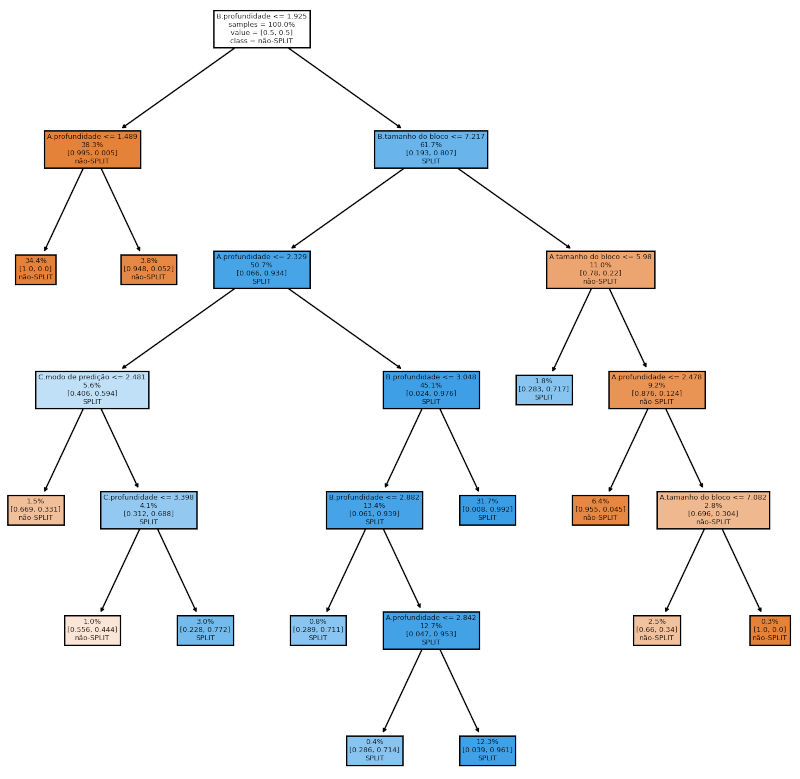
\includegraphics[width=\textwidth]{FIGURES/fig_34.png}
    \caption{Uma árvore de decisão gerada pelos modelos propostos. Fonte: Elaborada pelo autor.}
    \label{fig:34}
\end{figure}

Destes 12 modelos treinados com o conjunto completo de dados de treinamento, conforme explicitado na subseção \ref{cap:7.2.3}, e configurados conforme a Tabela \ref{tab:XXV}, foi possível obter os valores de F1-Score para todos os modelos e todas as propostas de transcodificador, conforme apresentados na Tabela \ref{tab:XXVI}. Nesta tabela, evidenciamos que a média obtida para a transcodificação de VP9 para AV1 é a maior de todas, apesar de que todas as demais apresentam valores muito próximos. Portanto, a expectativa é que os resultados de transcodificação sejam também próximos, principalmente relacionados ao impacto na eficiência da codificação. Analisando os resultados individuais de cada modelo presente na Tabela \ref{tab:XXVI}, é possível notar que o valor de \textit{F1-Score} decai conforme a profundidade aumenta. Por exemplo, o modelo do CQ 20 e profundidade 0 do transcodificador de H.266/VVC para AV1 possui um \textit{F1-Score} de 0,9929, enquanto que o modelo relacionado à profundidade 2 possui o valor de 0,9412. Apesar de ser uma diferença pequena, que se reflete em maior ou menor grau nos demais casos similares, hipotetiza-se que essa diferença implique em um erro de decisão maior nas sequências que requisitem uma profundidade maior da árvore de particionamento. Em outras palavras, vídeos que necessitem de maiores detalhes devem ter um impacto na eficiência de codificação maior que em sequências onde blocos grandes são mais utilizados, basicamente, em cenas mais paradas ou com grandes áreas homogêneas. 

\begin{table}
\begin{center}
\caption{Resultados da métrica \textit{F1-Score} obtidos com os modelos preditivos treinados sob os candidatos vencedores de cada proposta de transcodificação acelerado implementado.}
\label{tab:XXVI}
\footnotesize

\begin{tblr}{
    colspec = {l|r|r|r|r|r},
    hlines,
    row{even} = {gray9}
}
\hline
\textbf{Modelo do Conjunto} & \textbf{VP9} & \textbf{H.264/AVC} & \textbf{VP8} & \textbf{H.265/HEVC} & \textbf{H.266/VVC}\\
1 (CQ 20 P 0) & 0,9919 & 0,9917 & 0,9926 & 0,9928 & 0,9929\\
2 (CQ 20 P 1) & 0,9552 & 0,9796 & 0,9774 & 0,9551 & 0,9588\\
3 (CQ 20 P 2) & 0,9592 & 0,9362 & 0,9480 & 0,9480 & 0,9412\\
4 (CQ 32 P 0) & 0,9933 & 0,9928 & 0,9929 & 0,9933 & 0,9932\\
5 (CQ 32 P 1) & 0,9608 & 0,9560 & 0,9513 & 0,9554 & 0,9507\\
6 (CQ 32 P 2) & 0,9508 & 0,9535 & 0,9450 & 0,9520 & 0,9448\\
7 (CQ 43 P 0) & 0,9932 & 0,9931 & 0,9939 & 0,9930 & 0,9934\\
8 (CQ 43 P 1) & 0,9500 & 0,9447 & 0,9484 & 0,9520 & 0,9494\\
9 (CQ 43 P 2) & 0,9445 & 0,9418 & 0,9393 & 0,9419 & 0,9465\\
10 (CQ 55 P 0) & 0,9934 & 0,9935 & 0,9933 & 0,9934 & 0,9933\\
11(CQ 55 P 1) & 0,9591 & 0,9512 & 0,9552 & 0,9571 & 0,9465\\
12 (CQ 55 P 2) & 0,9330 & 0,9398 & 0,9344 & 0,9324 & 0,9389\\
\textbf{Média} & \textbf{0,9654} & \textbf{0,9645} & \textbf{0,9643} & \textbf{0,9639} & \textbf{0,9625}\\
\hline
\end{tblr}
\end{center}
\end{table}


Por fim, antes de apresentar os resultados obtidos, é preciso relembrar que a média de aceleração observada na literatura, conforme foi visto no capítulo \ref{cap:3}, é de 50,74\% de TS e de 4,11\% de BD-rate. Também ressaltamos neste capítulo que a comparação direta de qualquer solução com a média observada não pode ser feita de forma justa, haja visto a necessidade de se equiparar não apenas os formatos de transcodificação, como também as sequências utilizadas, as configurações aplicadas e a aplicabilidade alvo da proposta. Destacado essa injustiça ao se realizar qualquer comparação, nesta tese serão aplicadas comparações superficiais com a média, tendo em vista a ausência de melhores trabalhos para comparações. Ressalta-se, ainda, que mesmo propostas com valores com menor destaque ao observado na média da literatura não implicam diretamente em propostas ruins, pois, como já dissemos, quaisquer análises de resultados desconsideram contextos intrínsecos dos trabalhos desenvolvidos naquelas propostas, tampouco sobre os formatos de transcodificação utilizados. Dessa forma, apesar do uso de correlações com a média observada na literatura ter seu propósito de criar expectativas, essa análise não valida ou invalida quaisquer resultados.


\subsection{Transcodificação Rápida de VP9-para-AV1}
\label{cap:7.5.1}

A Tabela \ref{tab:XXVII} dispõe de todos os resultados obtidos para o transcodificador rápido de VP9 para AV1. Observa-se uma aceleração média da transcodificação de 16,76\%, a um custo de elevar o BD-rate em 5,10\%. Os três melhores resultados desta transcodificação estão na resolução HD1080, cuja resolução foi utilizado para realizar os treinamentos dos modelos preditivos. Nesta resolução em especial (HD1080), observa-se um TS de 19,58\% e um BD-rate de 4,47\%. As três sequências que apresentaram maior destaque são: \textit{crowd\_run\_1080p50\_60f}, \textit{ducks\_take\_off\_1080p50\_60f} e \textit{guitar\_hdr\_amazon\_1080p}, respectivamente com acelerações iguais a 36,81\%, 37,35\% e 51,96\%. Inclusive, a sequência \textit{guitar\_hdr\_amazon\_1080p} apresentou o maior TS entre todos os resultados de transcodificação rápida de VP9 para AV1. Apesar de serem sequências com cenas bem distintas (como pode ser visto no Apêndice \ref{apx:A}), indo desde patos nadando em um lago até um grupo de pessoas correndo montanha abaixo, há algo que é similar entre eles: são cenas de movimento em toda a área do quadro. Isso indica que as sequências devam usar uma quantidade maior de blocos menores, sugerindo que os modelos preditivos, pelo menos para as profundidades 0 e 1, são eficientes em predizer corretamente o particionamento do bloco.

\begin{center}
{\footnotesize
\begin{longtblr}[
    caption = {Resultados da transcodificação rápida de VP9 para AV1 baseado em modelos preditivos.},
    label = {tab:XXVII}
]{
    colspec = {l|p{6cm}|r|r|r},
    hlines,
    row{even} = {gray9}
}
\hline
\textbf{Resolução} & \textbf{Sequência} & \textbf{BD-rate (\%)} & \textbf{TS (\%)} & \textbf{Razão}\\
\SetCell[r=12]{l}HD720 & boat\_hdr\_amazon\_720p & 4,2537 & 13,99 & 0,304\\
 & dark720p\_120f & 5,4006 & 19,44 & 0,278\\
 & FourPeople\_1280x720\_60 & 2,4022 & 7,98 & 0,301\\
 & FourPeople\_1280x720\_60\_120f & 2,3122 & 8,05 & 0,287\\
 & gipsrestat720p\_120f & 2,6988 & 11,76 & 0,229\\
 & Johnny\_1280x720\_60 & 4,0714 & 14,33 & 0,284\\
 & Johnny\_1280x720\_60\_120f & 3,8174 & 15,76 & 0,242\\
 & KristenAndSara\_1280x720\_60 & 3,0265 & 16,69 & 0,181\\
 & KristenAndSara\_1280x720\_60\_120f & 3,0265 & 16,63 & 0,182\\
 & Netflix\_DinnerScene\_1280x720\_60fps \_8bit\_420\_120f & 6,3817 & 27,47 & 0,232\\
 & Netflix\_DrivingPOV\_1280x720\_60fps \_8bit\_420\_120f & 3,0173 & 12,54 & 0,241\\
 & Netflix\_FoodMarket2\_1280x720\_60fps \_8bit\_420\_120f & 2,966 & 8,99 & 0,330\\
\SetCell[r=8]{l}HD720 & Netflix\_RollerCoaster\_1280x720\_60fps \_8bit\_420\_120f & 5,7515 & 25,11 & 0,229\\
 & Netflix\_Tango\_1280x720\_60fps\_8bit \_420\_120f & 4,3562 & 8,07 & 0,540\\
 & rain\_hdr\_amazon\_720p & 1,0663 & 7,37 & 0,145\\
 & vidyo1\_720p\_60fps\_120f & 3,2613 & 12,9 & 0,253\\
 & Vidyo3\_1280x720\_60 & 3,8858 & 14,11 & 0,275\\
 & vidyo3\_720p\_60fps\_120f & 3,6996 & 14,16 & 0,261\\
 & Vidyo4\_1280x720\_60 & 2,9377 & 13,09 & 0,225\\
 & vidyo4\_720p\_60fps\_120f & 3,1043 & 12,99 & 0,239\\
\SetCell[c=2]{r}\textbf{Média dos vídeos HD720} && \textbf{3,5718} & \textbf{14,07} & \\
\SetCell[r=17]{l}HD1080 & aspen\_1080p\_60f & 5,7618 & 9,11 & 0,632\\
 & crowd\_run\_1080p50\_60f & 2,736 & 36,81 & 0,074\\
 & ducks\_take\_off\_1080p50\_60f & 4,4386 & 37,35 & 0,119\\
 & guitar\_hdr\_amazon\_1080p & 6,3438 & 51,96 & 0,122\\
 & Netflix\_Aerial\_1920x1080\_60fps\_8bit \_420\_60f & 4,2699 & 29,04 & 0,147\\
 & Netflix\_Boat\_1920x1080\_60fps\_8bit \_420\_60f & 1,7737 & 18,42 & 0,096\\
 & Netflix\_Crosswalk\_1920x1080\_60fps \_8bit\_420\_60f & 3,7432 & 24,88 & 0,150\\
 & Netflix\_FoodMarket\_1920x1080\_60fps \_8bit\_420\_60f & 4,862 & 12,47 & 0,390\\
 & Netflix\_PierSeaside\_1920x1080\_60fps \_8bit\_420\_60f & 3,9322 & 9,41 & 0,418\\
 & Netflix\_SquareAndTimelapse\_1920x 1080\_60fps\_8bit\_420\_60f & 3,7862 & 8,64 & 0,438\\
 & Netflix\_TunnelFlag\_1920x1080\_60fps \_8bit\_420\_60f & 7,6284 & 28,33 & 0,269\\
 & old\_town\_cross\_1080p50\_60f & 7,6534 & 16,34 & 0,468\\
 & park\_joy\_1080p50\_60f & 2,012 & 9,3 & 0,216\\
 & pedestrian\_area\_1080p25\_60f & 4,2314 & 9,42 & 0,449\\
 & rush\_field\_cuts\_1080p\_60f & 2,4349 & 14,08 & 0,173\\
 & rush\_hour\_1080p25\_60f & 4,5744 & 11,41 & 0,401\\
 & seaplane\_hdr\_amazon\_1080p & 3,1675 & 14,68 & 0,216\\
HD1080 & station2\_1080p25\_60f & 7,2066 & 10,69 & 0,674\\
\SetCell[c=2]{r}\textbf{Média dos vídeos HD1080} && \textbf{4,4753} & \textbf{19,58} & \\
\SetCell[r=6]{l}UHD4K & Netflix\_BoxingPractice\_4096x2160 \_60fps\_10bit\_420\_60f & 11,0334 & 18,01 & 0,613\\
 & Netflix\_Dancers\_4096x2160\_60fps \_10bit\_420\_60f & 24,0996 & 17,77 & 1,356\\
 & Netflix\_Narrator\_4096x2160\_60fps \_10bit\_420\_60f & 12,2722 & 22,98 & 0,534 \\
 & Netflix\_RitualDance\_4096x2160\_60fps \_10bit\_420\_60f & 14,1521 & 20,86 & 0,679 &  & \\
 & Netflix\_ToddlerFountain\_4096x2160 \_60fps\_10bit\_420\_60f & 2.8256 & 19,93 & 0,142 \\
 & Netflix\_WindAndNature\_4096x2160 \_60fps\_10bit\_420\_60f & 8,0698 & 3,96 & 2,038
 \\
\SetCell[c=2]{r}\textbf{Média dos vídeos UHD4K} && \textbf{12,0755} & \textbf{17,25}  & \\
\SetCell[c=2]{r}\textbf{Média Geral} && \textbf{5,1010} & \textbf{16,76} & \\
\SetCell[c=2]{r}\textbf{Desvio Padrão Geral} && \textbf{3,9862} & \textbf{9,30} & \\
\hline
\end{longtblr}
}
\end{center}



Se os resultados observados na resolução HD1080 apresentam resultados positivos em algumas condições, adaptar a proposta para uma resolução menor, como HD720, não trouxe impactos negativos. Inclusive, apresenta resultados similares de redução do tempo (média de 14,07\%) e de impacto na eficiência de codificação (média de 3,57\%) em relação aos resultados observados na resolução HD1080. Nesta resolução, a sequência com a menor Razão foi \textit{rain\_hdr\_amazon\_720p}, com 0,145 pontos, originários de uma aceleração de 7,37\% da transcodificação e um BD-rate de 1,06\%. A sequência HD720 que obteve o maior TS foi \textit{Netflix\_DinnerScene\_1280x720\_60fps\_8bit\_420\_120f} com 27,47\%, mas o BD-rate foi de 6,38\%. Coincidentemente, é com esta sequência de vídeo que se observa o maior BD-rate para a resolução HD720. Todavia, quase todos os vídeos UHD4K não apresentaram resultados satisfatórios de eficiência de codificação, com resultados de BD-rate superiores a 8\% e uma aceleração inferior à 22,98\% (vista na sequência \textit{Netflix\_Narrator\_4096x2160\_60fps\_10bit\_420\_60f}). A única exceção é \textit{Netflix\_ToddlerFountain\_4096x2160\_60fps\_10bit\_420\_60f}, que apresenta 2,82\% de BD-rate e 19,93\% de TS. 

Há, publicado na literatura científica, outra proposta de transcodificador rápido de VP9 para AV1, que desenvolvemos e apresentamos na seção \ref{cap:6.2}. Essa proposta apresentou uma redução de complexidade de 28,16\% a um custo na eficiência de codificação de 4,34\%. Essa proposta de transcodificador rápido não utiliza modelos preditivos para auxiliar nas decisões rápidas e, portanto, consegue apresentar uma média geral melhor que a proposta apresentada nesta subseção, baseada em modelos preditivos. Contudo, o trabalho descrito na seção \ref{cap:6.2} utiliza um conjunto menor de vídeos para avaliar os resultados, apesar de apresentar uma maior variedade de resoluções. Se considerarmos apenas as mesmas sequências utilizadas nas duas propostas, obteremos os dados apresentados na Tabela \ref{tab:XXVIII}, onde comparamos diretamente as duas propostas apresentadas nesta tese para a transcodificação rápida de VP9 para AV1.

\begin{table}
\begin{center}
\caption{Relação direta entre as propostas de transcodificador rápido do formato VP9 para o AV1.}
\label{tab:XXVIII}
\footnotesize

\begin{tblr}{
    colspec = {p{4cm}|r|r|r|r|r|r},
    hlines,
    row{even} = {gray9}
}
\hline
& \SetCell[c=3]{c}\textbf{Proposta com Modelos Preditivos} &&& \SetCell[c=3]{c}\textbf{Proposta com Heurística} &&\\
\textbf{Sequência} & \textbf{BD-rate (\%)} & \textbf{TS (\%)} & \textbf{Razão} & \textbf{BD-rate (\%)} & \textbf{TS (\%)} & \textbf{Razão} \\
dark720p\_120f & 5,40 & 19,44 & 0,28 & 4,14 & 23,02 & 0,18 \\
Johnny\_1280x720\_60\_ 120f & 3,82 & 15,76 & 0,24 & 6,05 & 24,74 & 0,24 \\
Netflix\_DrivingPOV\_1280x 720\_60fps\_8bit\_420\_120f & 3,02 & 12,54 & 0,24 & 6,37 & 31,58 & 0,20 \\
Netflix\_RollerCoaster\_ 1280x720\_60fps\_8bit\_420\_120f & 5,75 & 25,11 & 0,23 & 6,69 & 41,73 & 0,16 \\
\SetCell[c=1]{r}\textbf{Média da resolução HD720} & \textbf{4,50} & \textbf{18,21} & \textbf{0,25} & \textbf{5,81} & \textbf{30,27} & \textbf{0,19} \\
crowd\_run\_1080p50\_60f & 2,74 & 36,81 & 0,07 & 3,53 & 34,25 & 0,10 \\
Netflix\_Crosswalk\_1920x 1080\_60fps\_8bit\_420\_60f & 3,74 & 24,88 & 0,15 & 4,00 & 18,01 & 0,22 \\
park\_joy\_1080p50\_60f & 2,01 & 9,30 & 0,22 & 5,86 & 42,67 & 0,14 \\
seaplane\_hdr\_amazon\_ 1080p & 3,17 & 14,68 & 0,22 & 4,98 & 24,53 & 0,20 \\
\SetCell[c=1]{r}\textbf{Média da resolução HD1080} & \textbf{2,91} & \textbf{21,42} & \textbf{0,14} & \textbf{4,60} & \textbf{29,87} & \textbf{0,15} \\
\SetCell[c=1]{r}\textbf{Média Geral} & \textbf{3,71} & \textbf{19,81} & \textbf{0,19} & \textbf{5,20} & \textbf{30,07} & \textbf{0,17}\\
\hline
\end{tblr}
\end{center}
\end{table}


Na Tabela \ref{tab:XXVIII} podemos observar que o impacto na eficiência de codificação gerado pela proposta baseada em modelos preditivos é menor que o da proposta baseada em heurística. Isso significa que os modelos treinados geram decisões mais assertivas, principalmente na resolução HD1080 (2,91\% contra os 4,60\%). Observe que as sequências \textit{crowd\_run\_1080p50\_60f} e \textit{Netflix\_Crosswalk\_1920x1080\_60fps\_8bit\_420\_60f} apresentaram resultados melhores, tanto em BD-rate como em TS, ao utilizar a proposta baseada em modelos preditivos. Todavia, a aceleração geral obtida com as propostas usando modelos preditivos é menor, em especial para a sequência \textit{park\_joy\_1080p50\_60f}, que foi acelerada em 42,67\% na proposta da seção 6.2 contra os 9,30\% da proposta deste capítulo.

Desta forma, foi preciso investigar a causa do valor de TS inferior. Identificou-se que o algoritmo de transcodificação rápida proposto, em especial na manipulação das matrizes citadas na subseção \ref{cap:7.4.1}, consomem um tempo de processamento significativamente elevado no transcodificador. Avaliando a sequência de vídeo \textit{crowd\_run\_1080p50\_60f} sob o nível de quantização 20, na transcodificação original esta tarefa foi executada em 60.466 segundos (ou 16,8 horas), enquanto que na transcodificação rápida a mesma sequência de vídeo foi processada em 42.181 segundos (11,7 horas). Apesar de podermos perceber uma redução do custo computacional em 30\% nesta única sequência, observaram-se 2.974 segundos (49,6 minutos) do tempo do transcodificador dedicados ao algoritmo desenvolvido, isto é, 7,05\%. O mesmo se observou em outra sequência de vídeo (\textit{pan\_hdr\_amazon\_1080p}) sob um nível de quantização diferente (CQ 43), que codificou em 24.484 segundos na transcodificação original contra os 19.424 segundos na transcodificação rápida, ou seja, atingiu uma redução de 20\% do tempo. No entanto, foram necessários 1.344 segundos na execução do algoritmo, ou seja, 6.92\% do tempo total da codificação do \textit{libaom}. Casos similares puderam ser vistos em outras sequências sob níveis de quantização diferentes, com consumos de tempo próximos a 7\%.

Portanto, conclui-se que é possível obter resultados melhores de redução de tempo, caso o algoritmo desenvolvido seja otimizado, a um teto de 7\%, caso sua execução atinja o tempo real. Assim sendo, dos resultados médios de aceleração da resolução HD1080, apresentados na Tabela \ref{tab:XXVII} (de 19,58\%), seria possível estimar um resultado de TS máximo de 26,57\%.

\subsection{Transcodificação Rápida de H.264/AVC-para-AV1}
\label{cap:7.5.2}

A proposta de transcodificador rápido desenvolvida de VP9 para AV1 foi adaptada de H.264/AVC para AV1, utilizando o \textit{pipeline} de processamento. Utilizando as mesmas sequências de vídeo descritas anteriormente, exceto para vídeos UHD4K, foi possível obter uma aceleração da transcodificação de 25,05\% a um custo de reduzir a eficiência de codificação em 5,58\%, como é possível notar na Tabela \ref{tab:XXIX}. Uma observação geral que pode ser vista nesta proposta de transcodificador, em relação ao caso VP9 para AV1, é que os resultados foram melhores para a resolução HD720, ao invés da resolução HD1080. O TS médio obtido na resolução HD720 foi de 30,52\%, contra os 18,67\% da resolução HD1080. Inclusive, o impacto na eficiência de codificação também é menor na resolução HD720 (5,30\% contra 5,91\%). Como o formato H.264/AVC foi desenvolvido para lidar principalmente com resoluções HD720 ou inferiores, supõe-se que as demais informações dos atributos, além das médias de profundidades e de tamanho de bloco, possam contribuir mais para a tomada de decisão nessas resoluções, mesmo utilizando um modelo preditivo treinado para uma resolução maior.

\begin{center}
{\footnotesize
\begin{longtblr}[
 caption = {Resultados da transcodificação rápida de H.264/AVC para AV1 baseada em modelos preditivos.},
 label = {tab:XXIX}
]{
 colspec = {l|p{6cm}|r|r|r},
 hlines,
 row{even} = {gray9}
}
\hline
\textbf{Resolução} & \textbf{Sequência} & \textbf{BD-rate (\%)} & \textbf{TS (\%)} & \textbf{Razão}\\
\SetCell[r=21]{c}HD720 & boat\_hdr\_amazon\_720p & 0,7029 & 12,91 & 0,054 \\
 & dark720p\_120f & 9,1593 & 42,26 & 0,217 \\
 & FourPeople\_1280x720\_60 & 2,6325 & 32,32 & 0,081 \\
 & FourPeople\_1280x720\_60\_120f & 2,5755 & 32,47 & 0,079 \\
 & gipsrestat720p\_120f & 3,6448 & 40,85 & 0,089 \\
 & Johnny\_1280x720\_60 & 7,7357 & 48,34 & 0,160 \\
 & Johnny\_1280x720\_60\_120f & 8,0233 & 49,13 & 0,163 \\
 & KristenAndSara\_1280x720\_60 & 6,0619 & 47,96 & 0,126 \\
 & KristenAndSara\_1280x720\_60\_120f & 6,0619 & 47,97 & 0,126 \\
 & Netflix\_DinnerScene\_1280x720\_60fps \_8bit\_420\_120f & 13,0913 & 37,94 & 0,345 \\
 & Netflix\_DrivingPOV\_1280x720\_60fps \_8bit\_420\_120f & 4,3667 & 17,2 & 0,254 \\
 & Netflix\_FoodMarket2\_1280x720\_60fps \_8bit\_420\_120f & 4,0778 & 20,33 & 0,201 \\
 & Netflix\_RollerCoaster\_1280x720\_60fps \_8bit\_420\_120f & 6,7889 & 43,18 & 0,157 \\
 & Netflix\_Tango\_1280x720\_60fps\_8bit \_420\_120f & 4,3732 & 9,2 & 0,475 \\
 & rain\_hdr\_amazon\_720p & 0,5833 & 10,98 & 0,053 \\
 & Vidyo1\_1280x720\_60 & 4,1503 & 16,69 & 0,249 \\
 & vidyo1\_720p\_60fps\_120f & 3,9878 & 17,05 & 0,234 \\
 & Vidyo3\_1280x720\_60 & 2,8683 & 8,04 & 0,357 \\
 & vidyo3\_720p\_60fps\_120f & 2,3452 & 8,75 & 0,268 \\
 & Vidyo4\_1280x720\_60 & 9,1446 & 48,11 & 0,190 \\
 & vidyo4\_720p\_60fps\_120f & 8,9525 & 49,16 & 0,182 \\
\SetCell[c=2]{r}\textbf{Média dos vídeos HD720} && \textbf{5,3013} & \textbf{30,52} & \\
\SetCell[r=5]{c}HD1080 & aspen\_1080p\_60f & 15,1526 & 33,99 & 0,446 \\
 & crowd\_run\_1080p50\_60f & 0,8863 & 15,65 & 0,057 \\
 & ducks\_take\_off\_1080p50\_60f & 3,3596 & 25,83 & 0,130 \\
 & guitar\_hdr\_amazon\_1080p & 1,1848 & 12,73 & 0,095 \\
 & Netflix\_Aerial\_1920x1080\_60fps\_8bit \_420\_60f & 5,1584 & 20,96 & 0,246 \\
\SetCell[r=13]{c}HD1080 & Netflix\_Boat\_1920x1080\_60fps\_8bit \_420\_60f & 1,8815 & 20,37 & 0,092 \\
 & Netflix\_Crosswalk\_1920x1080\_60fps \_8bit\_420\_60f & 10,3418 & 12,52 & 0,826 \\
 & Netflix\_FoodMarket\_1920x1080\_60fps \_8bit\_420\_60f & 9,5122 & 19,58 & 0,486 \\
 & Netflix\_PierSeaside\_1920x1080\_60fps \_8bit\_420\_60f & 11,0504 & 41,32 & 0,267 \\
 & Netflix\_SquareAndTimelapse\_1920x 1080\_60fps\_8bit\_420\_60f & 3,0506 & 12,59 & 0,240 \\
 & Netflix\_TunnelFlag\_1920x1080\_60fps \_8bit\_420\_60f & 6,7701 & 17,9 & 0,380 \\
 & old\_town\_cross\_1080p50\_60f & 6,3312 & 21,54 & 0,294 \\
 & park\_joy\_1080p50\_60f & 1,0161 & 12,37 & 0,082 \\
 & pedestrian\_area\_1080p25\_60f & 8,176 & 14,23 & 0,575 \\
 & rush\_field\_cuts\_1080p\_60f & 1,0555 & 13,72 & 0,077 \\
 & rush\_hour\_1080p25\_60f & 8,4783 & 14,01 & 0,605 \\
 & seaplane\_hdr\_amazon\_1080p & 0,324 & 5,71 & 0,057 \\
 & station2\_1080p25\_60f & 12,7702 & 21,11 & 0,605 \\
\SetCell[c=2]{r}\textbf{Média dos vídeos HD1080} && \textbf{5,9166} & \textbf{18,67} & \\
\SetCell[c=2]{r}\textbf{Média Geral} && \textbf{5,5853} & \textbf{25,05} & \\
\SetCell[c=2]{r}\textbf{Desvio Padrão Geral} && \textbf{3,8649} & \textbf{14,28} & \\
\hline
\end{longtblr}
}
\end{center}



Os principais destaques na transcodificação de H.264/AVC para AV1 são para as sequências \textit{boat\_hdr\_amazon\_720p}, \textit{rain\_hdr\_amazon\_720p}, \textit{crowd\_run\_1080p50\_60f} e \textit{seaplane\_hdr\_amazon\_1080p}, todos com menos de 0,06 pontos de Razão. Uma característica entre essas sequências é que há uma metade da cena relativamente estática e outra com muitos movimentos, geralmente de água ou de pessoas distantes. Isso significa que há uma mescla homogênea entre tamanhos de bloco, o que, somado às demais informações extraídas dos atributos do H.264/AVC em relação ao VP9, pode impulsionar uma melhora significativa dos resultados observados nesta proposta de transcodificador rápido.

No entanto, há sete sequências HD1080 na Tabela \ref{tab:XXIX} que podem ser enquadradas como resultados negativos, sendo que quatro delas ultrapassam a marca de 10\% de BD-rate. Em especial \textit{Netflix\_Crosswalk\_1920x1080\_60fps\_8bit\_420\_60f}, que apresenta a maior Razão entre todas as sequências, com 12,52\% de TS e 10,34\% de BD-rate. Nota-se uma inversão completa em relação à proposta de VP9 para AV1, onde esta mesma sequência foi uma das de maior destaque, apresentando 24,88\% de TS e 3,74\% de BD-rate. Não identificamos uma causa para essa inversão específica.

Como visto na Tabela \ref{tab:III}, não há outros trabalhos de transcodificação de H.264/AVC para AV1. Portanto, esta é uma proposta inédita de transcodificador rápido e não existem comparações diretas que possam ser feitas. Todavia, observa-se uma média de aceleração dos trabalhos apresentados na literatura científica com o dobro do percentual apresentado do transcodificador apresentado neste subseção. Apesar de não ser possível fazer uma comparação justa dos resultados deste transcodificador rápido com a média da literatura, como já abordamos no Capítulo \ref{cap:3}, ainda assim a redução média de um quarto do tempo do transcodificador rápido, em relação ao transcodificador original, é um resultado positivo.

Considerando os valores de razão próximos ao apresentado pela proposta desenvolvida nesta subseção (de 0,13), os nossos resultados podem ser comparados diretamente com os valores obtidos por \citet{bib:peixoto_2012} (52,75\% de TS e 5,49\% de BD-rate), \citet{bib:peixoto2_2014} (74,54\% de TS e 8,41\% de BD-rate) e \citet{bib:franche_2017} (87,32\% de TS e 3,28\% de BD-rate). Destes trabalhos, \citet{bib:franche_2017} também utiliza informações provenientes tanto do decodificador como do codificador, apesar de sua proposta ser baseada em heurísticas. Por outro lado, \citet{bib:peixoto2_2014} propõe uma solução baseada em modelos preditivos gerados por \textit{Linear Discriminant Function} \cite{bib:shumway_1974}.

\subsection{Transcodificação Rápida de VP8-para-AV1}
\label{cap:7.5.3}

O formato de codificação de vídeo VP8 é o antecessor do formato VP9 e, como visto anteriormente nesta tese, possui uma série de limitações em comparação aos formatos mais recentes. Por exemplo, o VP8 só permite dois tamanhos de blocos, cada um voltado para um tipo de predição específico: interquadros (blocos de 16$\times$16) e intraquadro (blocos de 4$\times$4). Além disso, o formato não tem a capacidade de trabalhar com vídeos HDR e nem com subamostragem diferente de 4:2:0. Tais limitações e diferenças significativas do  formato VP8, explicam, em parte, os resultados obtidos na Tabela \ref{tab:XXXI}. Nesta tabela, observamos que a proposta de transcodificador rápido de VP8 para AV1, baseado em modelos preditivos, atinge uma aceleração de 55,69\% em relação ao transcodificador original, a melhor média de TS dentre todas as propostas desta tese e similar ao observado na literatura. No entanto, a solução impacta a eficiência de codificação em 12,85\% de BD-rate e, mesmo assim, ainda é uma solução inédita na literatura.

\begin{center}
{\footnotesize
\begin{longtblr}[
    caption = {Resultados obtidos com a transcodificação acelerada de VP8-para-AV1.},
    label = {tab:XXXI}
]{
    colspec = {l|p{6cm}|r|r|r},
    hlines,
    row{even} = {gray9},
    cell{10}{1} = {white},
    cell{34}{1} = {white}
}
\hline
\textbf{Resolução} & \textbf{Sequência} & \textbf{BD-rate (\%)} & \textbf{TS (\%)} & \textbf{Razão}\\
\SetCell[r=19]{c}HD720 & dark720p\_120f & 23,1199 & 76,25 & 0,303\\
 & FourPeople\_1280x720\_60 & 6,4063 & 71,03 & 0,090\\
 & FourPeople\_1280x720\_60\_120f & 6,5943 & 70,76 & 0,093\\
 & gipsrestat720p\_120f & 10,7597 & 77,57 & 0,139\\
 & Johnny\_1280x720\_60 & 16,2512 & 79,12 & 0,205\\
 & Johnny\_1280x720\_60\_120f & 16,2456 & 79,7 & 0,204\\
 & KristenAndSara\_1280x720\_60 & 13,4166 & 80,78 & 0,166\\
 & KristenAndSara\_1280x720\_60\_120f & 13,4166 & 80,87 & 0,166\\
 & Netflix\_DinnerScene\_1280x720\_60fps \_8bit\_420\_120f & 25,6688 & 62,58 & 0,410\\
 & Netflix\_DrivingPOV\_1280x720\_60fps \_8bit\_420\_120f & 10,9251 & 64,91 & 0,168\\
 & Netflix\_FoodMarket2\_1280x720\_60fps \_8bit\_420\_120f & 8,0288 & 34,59 & 0,232\\
 & Netflix\_RollerCoaster\_1280x720\_60fps \_8bit\_420\_120f & 15,327 & 66,61 & 0,230\\
 & Netflix\_Tango\_1280x720\_60fps\_8bit \_420\_120f & 7,5238 & 21,39 & 0,352\\
 & Vidyo1\_1280x720\_60 & 6,563 & 23,72 & 0,277\\
 & vidyo1\_720p\_60fps\_120f & 6,3635 & 24,61 & 0,259\\
 & Vidyo3\_1280x720\_60 & 11,6042 & 73,5 & 0,158\\
 & vidyo3\_720p\_60fps\_120f & 10,8592 & 73,31 & 0,148\\
 & Vidyo4\_1280x720\_60 & 16,2467 & 76,42 & 0,213\\
 & vidyo4\_720p\_60fps\_120f & 16,0305 & 76,03 & 0,211\\
\SetCell[c=2]{r}\textbf{Média dos vídeos HD720} && \textbf{12,7027} & \textbf{63,88} & \\
\SetCell[r=6]{c}HD1080 & aspen\_1080p\_60f & 24,1958 & 29,86 & 0,810\\
 & crowd\_run\_1080p50\_60f & 1,5514 & 30,57 & 0,051\\
 & ducks\_take\_off\_1080p50\_60f & 4,4886 & 49,62 & 0,090\\
 & Netflix\_Aerial\_1920x1080\_60fps\_8bit \_420\_60f & 10,7455 & 37,82 & 0,284\\
 & Netflix\_Boat\_1920x1080\_60fps\_8bit \_420\_60f & 2,8285 & 31,87 & 0,089\\
 & Netflix\_Crosswalk\_1920x1080\_60fps \_8bit\_420\_60f & 23,1568 & 32,74 & 0,707\\
\SetCell[r=10]{c}HD1080 & Netflix\_FoodMarket\_1920x1080\_60fps \_8bit\_420\_60f & 16,0831 & 32,88 & 0,489\\
 & Netflix\_PierSeaside\_1920x1080\_60fps \_8bit\_420\_60f & 14,2656 & 76,93 & 0,185\\
 & Netflix\_SquareAndTimelapse\_1920x 1080\_60fps\_8bit\_420\_60f & 4,9242 & 26,52 & 0,186\\
 & Netflix\_TunnelFlag\_1920x1080\_60fps \_8bit\_420\_60f & 11,5801 & 33,64 & 0,344\\
 & old\_town\_cross\_1080p50\_60f & 20,4893 & 76,59 & 0,268\\
 & park\_joy\_1080p50\_60f & 2,2236 & 54,74 & 0,041\\
 & pedestrian\_area\_1080p25\_60f & 22,9798 & 72,67 & 0,316\\
 & rush\_field\_cuts\_1080p\_60f & 1,9172 & 30,92 & 0,062\\
 & rush\_hour\_1080p25\_60f & 22,3852 & 75,96 & 0,295\\
 & station2\_1080p25\_60f & 24,689 & 42,05 & 0,587\\
\SetCell[c=2]{r}\textbf{Média dos vídeos HD1080} && \textbf{13,0315} & \textbf{45,96} & \\
\SetCell[c=2]{r}\textbf{Média Geral} && \textbf{12,853} & \textbf{55,69} & \\
\SetCell[c=2]{r}\textbf{Desvio Padrão Geral} && \textbf{7,2509} & \textbf{21,75} & \\
\hline
\end{longtblr}
}
\end{center}



Embora os resultados médios não sejam positivos em termos de eficiência de codificação, principalmente quando comparamos com a média da literatura, alguns destaques podem ser feitos, principalmente quanto à resolução HD1080. As três sequências de menor BD-rate são \textit{crowd\_run\_1080p50\_60f}, \textit{rush\_field\_cuts\_1080p\_60f} e \textit{park\_joy\_1080p50\_60f}, com respectivamente 1,55\%, 1,91\% e 2,22\% de BD-rate e com reduções de complexidade de 30,57\% 30,92\% e 54,74\%. Não encontrou-se uma similaridade direta entre essas três sequências. No entanto, após uma investigação avaliando outras características dos vídeos, percebeu-se que todos são vídeos com uma grande taxa de informação espacial (do inglês, \textit{Spatial Information}, SI). Conforme podemos ver na descrição das sequências no Apêndice \ref{apx:A}, as seis sequências HD1080 com mais de 60 pontos de SI são, em ordem crescente: \textit{ducks\_take\_off\_1080p50\_60f}, \textit{rush\_field\_cuts\_1080p\_60f}, \textit{Netflix\_Boat\_1920x1080\_60fps\_8bit\_420\_60f}, \textit{Netflix\_TunnelFlag\_1920x1080\_60fps\_8bit\_420\_60f}, \textit{park\_joy\_1080p50\_60f} e \textit{crowd\_run\_1080p50\_60f}. Destas, apenas a sequência \textit{Netflix\_TunnelFlag\_1920x1080\_60fps\_8bit\_420\_60f} apresenta resultados ruins para a solução proposta.

A sequência com a maior Razão é \textit{aspen\_1080p\_60f}. Observando os resultados de codificação dessa sequência, notamos uma perda de PSNR de -1,067dB no nível de quantização 55. Essa perda de qualidade somada ao aumento de 41,6\% da taxa de bits de \textit{aspen\_1080p\_60f} nesse nível de quantização, justificam o BD-rate de 24,19\%. Para exemplificar essa diferença de PSNR, apresentamos na Figura \ref{fig:35} uma parte de maior destaque do último quadro da sequência \textit{aspen\_1080p\_60f}. sob o nível de quantização 55. Os quadros apresentados na Figura \ref{fig:35} estão em diferentes momentos: Figura \ref{fig:35}(a) apresenta o quadro original, sem compressão seguido pela sua aparência após a decodificação do VP8 (Figura \ref{fig:35}(b)). Na Figura \ref{fig:35}(c) apresenta o quadro codificado pelo transcodificador original e Figura \ref{fig:35}(d) apresenta o quadro codificado pelo transcodificador rápido. Como é possível observar nestas figuras, nota-se uma perda da nitidez das folhas, em especial do interior delas. Apesar das ranhuras e das manchas da folha se perderem um pouco após a codificação por parte do VP8, ainda é possível percebê-las após a decodificação (Figura \ref{fig:35}(b)). Todavia, após a transcodificação para o AV1, quase todas as ranhuras se perdem, em especial quando transcodificadas pela nossa proposta rápida, restando na cena um borrão verde. E apesar da sequência \textit{aspen\_1080p\_60f}, assim como a maioria das sequências com BD-rate acima dos 20\%, também serem sequências com valores negativos na transcodificação de H.264/AVC para AV1, não foi possível identificar alguma característica intrínseca ao vídeo que auxiliasse na explicação desses valores elevados de BD-rate.

\begin{figure}
    \centering
    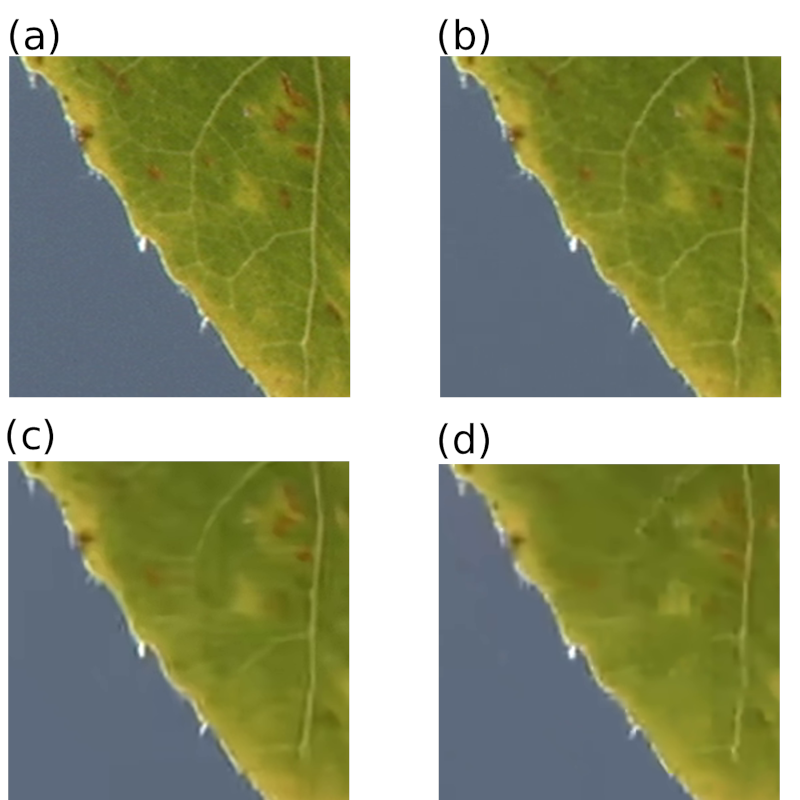
\includegraphics[width=\textwidth]{FIGURES/fig_35.png}
    \caption{Destaque do último quadro do vídeo \textit{aspen\_1080p\_60f} para as sequências (a) original, (b) decodificada pelo VP8, (c) transcodificada original para o AV1 e (d) transcodificada acelerada para o AV1. Fonte: Elaborada pelo autor.}
    \label{fig:35}
\end{figure}


\subsection{Transcodificação Rápida de H.265/HEVC-para-AV1}
\label{cap:7.5.4}

A Tabela \ref{tab:XXXIII} apresenta os resultados obtidos com a transcodificação rápida de H.265/HEVC para AV1, cujo algoritmo foi desenvolvido seguindo a mesma metodologia da proposta de VP9 para AV1. Nesta tabela, é possível observar que a solução é capaz de atingir uma aceleração da transcodificação de 28,36\%, a um custo de 6,74\% de BD-rate. A sequência de maior destaque é \textit{ducks\_take\_off\_1080p50\_60f}, com 41,64\% de TS e 4,10\% de BD-rate. Assim como os resultados de H.264/AVC e de VP8, na proposta para o H.265/HEVC observa-se uma maior redução de tempo nas sequências HD720 do que nas sequências HD1080, para os quais os modelos foram treinados. O fato de só haver uma única sequência HD720 que é caso destacadamente negativa (\textit{dark720p\_120f}), contra os cinco exemplos da resolução HD1080 (\textit{Netflix\_Aerial\_1920x1080\_60fps\_8bit\_420\_60f}, \textit{Netflix\_Crosswalk\_1920x1080\_60fps\_8bit\_420\_60f}, \textit{Netflix\_FoodMarket\_1920x1080\_60fps\_8bit\_420\_60f}, \textit{pedestrian\_area\_1080p25\_60f} e \textit{station2\_1080p25\_60f}) conta bastante para essa diferença em favor da resolução menor, mesmo que pequena. Outro ponto de destaque na proposta de H.265/HEVC para AV1 é que, diferentemente do que observamos no transcodificador rápido de VP9 para AV1, os resultados obtidos na transcodificação de vídeos UHD4K não são compostos por casos negativos. Apesar da baixa aceleração obtida, todos possuem valores de BD-rate baixos (menos de 3,2\%). Isso indica que as amostras geradas pelo decodificador H.265/HEVC em vídeos UHD4K fornecem dados mais confiáveis e de maior qualidade que os gerados pelo decodificador VP9.

\begin{center}
{\footnotesize
\begin{longtblr}[
    caption = {Resultados da transcodificação rápida de H.265/HEVC para AV1 baseado em modelos preditivos.},
    label = {tab:XXXIII}
]{
    colspec = {l|p{6cm}|r|r|r},
    hlines,
    row{even} = {gray9},
    cell{23}{1} = {gray9},
    cell{42}{1} = {white},
}
\hline
\textbf{Resolução} & \textbf{Sequência} & \textbf{BD-rate (\%)} & \textbf{TS (\%)} & \textbf{Razão}\\
\SetCell[r=20]{l}HD720 & boat\_hdr\_amazon\_720p & 4,2537 & 13,99 & 0,304\\
 & dark720p\_120f & 5,4006 & 19,44 & 0,278\\
 & FourPeople\_1280x720\_60 & 2,4022 & 7,98 & 0,301\\
 & FourPeople\_1280x720\_60\_120f & 2,3122 & 8,05 & 0,287\\
 & gipsrestat720p\_120f & 2,6988 & 11,76 & 0,229\\
 & Johnny\_1280x720\_60 & 4,0714 & 14,33 & 0,284\\
 & Johnny\_1280x720\_60\_120f & 3,8174 & 15,76 & 0,242\\
 & KristenAndSara\_1280x720\_60 & 3,0265 & 16,69 & 0,181\\
 & KristenAndSara\_1280x720\_60\_120f & 3,0265 & 16,63 & 0,182\\
 & Netflix\_DinnerScene\_1280x720\_60fps \_8bit\_420\_120f & 6,3817 & 27,47 & 0,232\\
 & Netflix\_DrivingPOV\_1280x720\_60fps \_8bit\_420\_120f & 3,0173 & 12,54 & 0,241\\
 & Netflix\_FoodMarket2\_1280x720\_60fps \_8bit\_420\_120f & 2,966 & 8,99 & 0,330\\
 & Netflix\_RollerCoaster\_1280x720\_60fps \_8bit\_420\_120f & 5,7515 & 25,11 & 0,229\\
 & Netflix\_Tango\_1280x720\_60fps\_8bit \_420\_120f & 4,3562 & 8,07 & 0,540\\
 & rain\_hdr\_amazon\_720p & 1,0663 & 7,37 & 0,145\\
 & vidyo1\_720p\_60fps\_120f & 3,2613 & 12,9 & 0,253\\
 & Vidyo3\_1280x720\_60 & 3,8858 & 14,11 & 0,275\\
 & vidyo3\_720p\_60fps\_120f & 3,6996 & 14,16 & 0,261\\
 & Vidyo4\_1280x720\_60 & 2,9377 & 13,09 & 0,225\\
 & vidyo4\_720p\_60fps\_120f & 3,1043 & 12,99 & 0,239\\
\SetCell[c=2]{r}\textbf{Média dos vídeos HD720} && \textbf{3,5718} & \textbf{14,07} & \\
\SetCell[r=4]{l}HD1080 & aspen\_1080p\_60f & 5,7618 & 9,11 & 0,632\\
 & crowd\_run\_1080p50\_60f & 2,736 & 36,81 & 0,074\\
 & ducks\_take\_off\_1080p50\_60f & 4,4386 & 37,35 & 0,119\\
 & guitar\_hdr\_amazon\_1080p & 6,3438 & 51,96 & 0,122\\
\SetCell[r=14]{l}HD1080 & Netflix\_Aerial\_1920x1080\_60fps\_8bit \_420\_60f & 4,2699 & 29,04 & 0,147\\
 & Netflix\_Boat\_1920x1080\_60fps\_8bit \_420\_60f & 1,7737 & 18,42 & 0,096\\
 & Netflix\_Crosswalk\_1920x1080\_60fps \_8bit\_420\_60f & 3,7432 & 24,88 & 0,150\\
 & Netflix\_FoodMarket\_1920x1080\_60fps \_8bit\_420\_60f & 4,862 & 12,47 & 0,390\\
 & Netflix\_PierSeaside\_1920x1080\_60fps \_8bit\_420\_60f & 3,9322 & 9,41 & 0,418\\
 & Netflix\_SquareAndTimelapse\_1920x 1080\_60fps\_8bit\_420\_60f & 3,7862 & 8,64 & 0,438\\
 & Netflix\_TunnelFlag\_1920x1080\_60fps \_8bit\_420\_60f & 7,6284 & 28,33 & 0,269\\
 & old\_town\_cross\_1080p50\_60f & 7,6534 & 16,34 & 0,468\\
 & park\_joy\_1080p50\_60f & 2,012 & 9,3 & 0,216\\
 & pedestrian\_area\_1080p25\_60f & 4,2314 & 9,42 & 0,449\\
 & rush\_field\_cuts\_1080p\_60f & 2,4349 & 14,08 & 0,173\\
 & rush\_hour\_1080p25\_60f & 4,5744 & 11,41 & 0,401\\
 & seaplane\_hdr\_amazon\_1080p & 3,1675 & 14,68 & 0,216\\
 & station2\_1080p25\_60f & 7,2066 & 10,69 & 0,674\\
\SetCell[c=2]{r}\textbf{Média dos vídeos HD1080} && \textbf{4,4753} & \textbf{19,58} & \\
\SetCell[r=3]{l}UHD4K & Netflix\_BarScene\_4096x2160\_60fps \_10bit\_420\_60f & 3,2829 & 15,88 & 0,207 \\
 & Netflix\_BoxingPractice\_4096x2160 \_60fps\_10bit\_420\_60f & 0,6495 & 11,07 & 0,059\\
 & Netflix\_Dancers\_4096x2160\_60fps \_10bit\_420\_60f & 1,6817 & 11,30 & 0,149\\
\SetCell[c=2]{r}\textbf{Média dos vídeos UHD4K} && \textbf{1,8714} & \textbf{12,75} & \\
\SetCell[c=2]{r}\textbf{Média Geral} && \textbf{6,7454} & \textbf{28,36} & \\
\SetCell[c=2]{r}\textbf{Desvio Padrão Geral} && \textbf{5,0544} & \textbf{15,90} & \\
\hline
\end{longtblr}
}
\end{center}



Há sete sequências que atingem um TS superior à 50\%, sendo que o de maior aceleração dentre eles é o \textit{Netflix\_RollerCoaster\_1280x720\_60fps\_8bit\_420\_120f}, com 55,26\% de TS. No entanto, todos possuem um BD-rate elevado, de aproximadamente 10\%. Por outro lado, a sequência \textit{seaplane\_hdr\_amazon\_1080p} é a que apresenta o menor BD-rate, com apenas 0,02\%. No entanto, também é a sequência com o menor TS de todo o conjunto de vídeos (0,47\%). Inclusive, quase todos os resultados obtidos com a solução H.265/HEVC para AV1 são próximos dos obtidos com a solução H.264/AVC para AV1, variando entre 2\% de BD-rate, para mais ou para menos. Há exceções (13 de 38 sequências, para ser preciso), cujos os dois maiores destaques são para \textit{dark720p\_120f}, que apresenta 15,33\% de BD-rate e 21,91\% de TS no H.265/HEVC contra os 9,15\% e 42,26\% no H.264/AVC; e a sequência \textit{old\_town\_cross\_1080p50\_60f} que obteve 14,05\% de BD-rate e 33,27\% de TS contra os 6,33\% de BD-rate e 21,54\% de TS. 

Não foi encontrado nenhuma relação entre os casos excepcionais que justificasse essa diferença nos resultados, assim como outra relação observada na Tabela \ref{tab:XXXIII}, de que todas as sequências HD1080 com 10 bits de profundidade (HDR) obtiveram um BD-rate inferior a 1\% e, ao mesmo tempo, são os vídeos com menor taxa de aceleração observada.

Há, na literatura científica, outros trabalhos que propõem soluções de transcodificação rápida de H.265/HEVC para AV1, os quais já foram apresentados na seção \ref{cap:6.1}. Além da nossa proposta desenvolvida na seção \ref{cap:6.1}, que apresenta resultados desde TS acima de 50\% ($La$:$Lb$ de 0:0, com 61,20\% de TS e 14,66\% de BD-rate) até menos de 5\% (por exemplo, $La$:$Lb$ de 4:2, com 4,60\% de TS e 0,0583\% de BD-rate), há o trabalho de \citet{bib:chen_2019}, com resultados de redução de TS em 37,8\% a um custo de 0,79\% do BD-rate. Apesar do resultado médio de TS observado na Tabela \ref{tab:XXXIII}, de 28,36\%, ser próximo ao do trabalho de \citet{bib:chen_2019}, inclusive com algumas sequências se aproximando da Razão apresentada por \citeauthor{bib:chen_2019} (de 0,021 pontos), no entanto, o BD-rate apresentado pelo nosso modelo é em ordens de grandeza diferentes.

Observa-se com a comparação da nossa proposta baseada em modelos preditivos com a proposta baseada em heurística, que os resultados médios se aproximam dos observados para a combinação $La$:$Lb$ iguais à 0:1, que apresenta um TS de 32\% e um BD-rate de 6,16\%. Ou senão, avaliando as razões de $La$:$Lb$, a solução proposta neste capítulo se aproxima dos resultados obtidos pelas combinações 0:3 (TS de 15,40\% e BD-rate de 3,58\%), 0:4 (TS de 15,10\% e BD-rate de 3,51\%) e 0:0 (TS de 61,20\% e BD-rate de 14,66\%), contudo, com resultados proporcionalmente melhores.

\subsection{Transcodificação Rápida de H.266/VVC-para-AV1}
\label{cap:7.5.5}

O formato de codificação de vídeo H.266/VVC é sucessor direto dos formatos H.265/HEVC e H.264/AVC. Assim sendo, espera-se observar resultados de redução de tempo similares. No entanto, ao observar os resultados de transcodificação na Tabela \ref{tab:XXXV}, notamos uma aceleração de apenas 12,05\%, mas acompanhado de uma redução considerável no impacto da eficiência de codificação, em relação às outras propostas apresentadas nesta tese, de apenas 1,67\% de BD-rate. O maior BD-rate foi atingido pela sequência \textit{dark720p\_120f}, com 6,12\%, que também apresenta a segunda maior aceleração da transcodificação de H.266/VVC para AV1, de 28,20\%.

\begin{table}
\begin{center}
\caption{Resultados HD1080 da transcodificação rápida de H.266/VVC para AV1 baseado em modelos preditivos.}
\label{tab:XXXV}
\footnotesize

\begin{tblr}{
    colspec = {l|p{6cm}|r|r|r},
    hlines,
    row{even} = {gray9}
}
\hline
\textbf{Resolução} & \textbf{Sequência} & \textbf{BD-rate (\%)} & \textbf{TS (\%)} & \textbf{Razão}\\
\SetCell[r=10]{c}1280$\times$720 & boat\_hdr\_amazon\_720p & 0,3002 & 5,42 & 0,055\\
& dark720p\_120f & 6,1287 & 28,20 & 0,217\\
& FourPeople\_1280x720\_60 & 1,1114 & 7,08 & 0,157\\
& Johnny\_1280x720\_60 & 1,9670 & 10,66 & 0,185\\
& Johnny\_1280x720\_60\_120f & 1,5881 & 33,49 & 0,047\\
& KristenAndSara\_1280x720\_60 & 1,0139 & 9,65 & 0,105\\
& Netflix\_DinnerScene\_1280x720\_60fps \_8bit\_420\_120f & 2,7381 & 2,38 & 1,152\\
& Netflix\_RollerCoaster\_1280x720\_60fps \_8bit\_420\_120f & 1,8403 & 14,84 & 0,124\\
& Netflix\_Tango\_1280x720\_60fps\_8bit \_420\_120f & 1,7705 & 10,73 & 0,165\\
& Vidyo4\_1280x720\_60 & 1,2974 & 11,59 & 0,112\\
\SetCell[c=2]{r}\textbf{Média dos vídeos HD720} && \textbf{1,9756} & \textbf{13,40} & \\
\SetCell[r=16]{c}1920$\times$1080 & aspen\_1080p\_60f & 4,0270 & 18,02 & 0,224\\
& crowd\_run\_1080p50\_60f & 0,4774 & 6,63 & 0,072\\
& ducks\_take\_off\_1080p50\_60f & 1,9142 & 22,52 & 0,085\\
& guitar\_hdr\_amazon\_1080p & 0,2210 & 0,74 & 0,300\\
& Netflix\_Boat\_1920x1080\_60fps\_8bit \_420\_60f & 0,4828 & 8,62 & 0,056\\
& Netflix\_Crosswalk\_1920x1080\_60fps \_8bit\_420\_60f & 2,0820 & 6,65 & 0,313\\
& Netflix\_FoodMarket\_1920x1080\_60fps \_8bit\_420\_60f & 2,7500 & 8,51 & 0,323\\
& Netflix\_PierSeaside\_1920x1080\_60fps \_8bit\_420\_60f & 1,6240 & 12,73 & 0,128\\
& Netflix\_SquareAndTimelapse\_1920x 1080\_60fps\_8bit\_420\_60f & 0,8282 & 7,96 & 0,104\\
& Netflix\_TunnelFlag\_1920x1080\_60fps \_8bit\_420\_60f & 2,1780 & 20,67 & 0,105\\
& pan\_hdr\_amazon\_1080p & 0,2280 & 0,05 & 4,367\\
& park\_joy\_1080p50\_60f & 0,3980 & 13,85 & 0,029\\
& pedestrian\_area\_1080p25\_60f & 2,4390 & 7,35 & 0,332\\
& rush\_field\_cuts\_1080p\_60f & 0,6430 & 16,46 & 0,039\\
& rush\_hour\_1080p25\_60f & 3,4070 & 25,63 & 0,133\\
& seaplane\_hdr\_amazon\_1080p & 0,1260 & 2,93 & 0,043\\
\SetCell[c=2]{r}\textbf{Média dos vídeos HD1080} && \textbf{1,4891} & \textbf{11,21} & \\
\SetCell[c=2]{r}\textbf{Média Geral} && \textbf{1,6762} & \textbf{12,05} & \\
\SetCell[c=2]{r}\textbf{Desvio Padrão Geral} && \textbf{1,3785} & \textbf{8,49} & \\
\hline
\end{tblr}
\end{center}
\end{table}


Apesar da média de aceleração obtida pela transcodificação H.266/VVC para AV1 ser a menor, principalmente em relação aos padrões antecessores do H.266/VVC, o qual se esperava uma aceleração similar, o BD-rate obtido também foi o menor de todos os cinco transcodificadores propostos baseados em aprendizado de máquina. Observe que o \textit{F1-Score} médio dos modelos deste transcodificador (H.266/VVC para AV1) são os menores em relação a todos apresentados na Tabela \ref{tab:XXVI} e, mesmo assim, o BD-rate obtido pelo transcodificador é o menor de todos.

Não há na literatura científica um trabalho de transcodificação rápida de H.266/VVC para AV1, e apesar de haver outros trabalhos de transcodificadores rápidos com os antecessores do H.266/VVC, não é válido utilizá-los como comparação direta. Dos trabalhos existentes na literatura, apenas \citet{bib:lucas_2020} também utiliza o H.266/VVC, mas propondo uma transcodificação rápida de H.265/HEVC para H.266/VVC. Ou seja, \citet{bib:lucas_2020} propõe utilizar o H.266/VVC como formato destino; em contrapartida, nós propomos que o formato H.266/VVC seja o formato de origem. \cite{bib:lucas_2020} propõe utilizar um modelo treinado pelo algoritmo Naïve-Bayes para acelerar o particionamento de blocos 128$\times$128. Com isso, observa-se uma aceleração de 13,38\%, a um custo na eficiência de codificação de 0,32\% de BD-rate. Observa-se que ambas as propostas, a nossa e a de \citet{bib:lucas_2020}, apresentam baixos valores de TS e BD-rate.

Todavia, assim como destacamos sobre comparações entre as soluções propostas com a média observada na literatura, é importante ressaltar que não é possível realizar uma comparação direta entre a proposta de \citet{bib:lucas_2020} à solução apresentada nesta tese, pois são propostas baseadas em diferentes padrões e implementações de codificadores.

\subsection{Considerações Gerais e Análise do \textit{Pipeline} de Processamento}
\label{cap:7.5.6}

Nas subseções anteriores apresentamos todas as cinco propostas de transcodificador rápido usando modelos preditivos, sendo que o \textit{pipeline} de processamento foi desenvolvido para a geração de modelos para o transcodificador de VP9 para AV1 e depois adaptando para gerar modelos para outros transcodificadores com diferentes formatos de origem: H.264/AVC, VP8, H.265/HEVC e H.266/VVC. Tendo como base as mesmas sequências utilizadas para geração dos dados de treinamento e teste, vimos que o \textit{F1-Score} médio dos 12 modelos tende a superar os 0,96 pontos. Considerando algumas limitações de cada experimento, foram disponibilizadas as mesmas sequências para uso na fase preditiva dos modelos, o que possibilitou a geração dos dados comparativos entre o transcodificador original e a proposta de transcodificador rápido. No entanto, houve diferenças de sequências finalizadas em cada uma das propostas. Visando possibilitar uma comparação mais justa entre as cinco propostas de transcodificador rápido baseado em modelos preditivos, a Tabela \ref{tab:XXXVI} apresenta uma visão geral das cinco propostas, contudo, considerando as mesmas sequências de vídeo que estão presente em todas elas.

\afterpage{
\clearpage

\begin{landscape}
\begin{center}
{\footnotesize
\begin{longtblr}[
 caption = {Resumo dos resultados das propostas de transcodificadores rápidos para o formato AV1.},
 label = {tab:XXXVI}
]{ 
 colspec = {lp{5.5cm}|rrrrrrrrrr},
 rowhead = 2,
 hlines,
 row{even} = {gray9},
 cell{3}{1} = {gray9},
 cell{17}{1} = {gray9}
}
\hline
\SetCell[r=2]{c} & \SetCell[r=2]{c}\textbf{Sequência} & \SetCell[c=2]{c}\textbf{VP9} && \SetCell[c=2]{c}\textbf{H.264/AVC} && \SetCell[c=2]{c}\textbf{VP8} && \SetCell[c=2]{c}\textbf{H.265/HEVC} && \SetCell[c=2]{c}\textbf{H.266/VVC} \\
& & BD-rate (\%) & TS (\%) & BD-rate (\%) & TS (\%) & BD-rate (\%) & TS (\%) & BD-rate (\%) & TS (\%) & BD-rate (\%) & TS (\%) \\
\SetCell[r=9]{c}\rotatebox[origin=c]{90}{1280$\times$720} & dark720p\_120f & 5,40 & 19,44 & 9,16 & 42,26 & 23,12 & 76,25 & 15,33 & 21,91 & 6,13 & 28,20 \\
& FourPeople\_1280x720\_60 & 2,40 & 7,98 & 2,63 & 32,32 & 6,41 & 71,03 & 3,40 & 16,54 & 1,11 & 7,08 \\
& Johnny\_1280x720\_60 & 4,07 & 14,33 & 7,74 & 48,34 & 16,25 & 79,12 & 9,71 & 55,15 & 1,97 & 10,66 \\
& Johnny\_1280x720\_60\_120f & 3,82 & 15,76 & 8,02 & 49,13 & 16,25 & 79,70 & 9,04 & 52,35 & 1,59 & 33,49 \\
& KristenAndSara\_1280x720\_60 & 3,03 & 16,69 & 6,06 & 47,96 & 13,42 & 80,78 & 7,62 & 52,93 & 1,01 & 9,65 \\
& Netflix\_DinnerScene\_1280x720\_ 60fps\_8bit\_420\_120f & 6,38 & 27,47 & 13,09 & 37,94 & 25,67 & 62,58 & 14,35 & 47,47 & 2,74 & 2,38 \\
& Netflix\_RollerCoaster\_1280x720\_ 60fps\_8bit\_420\_120f & 5,75 & 25,11 & 6,79 & 43,18 & 15,33 & 66,61 & 11,35 & 55,26 & 1,84 & 14,84 \\
& Netflix\_Tango\_1280x720\_60fps\_8bit \_420\_120f & 4,36 & 8,07 & 4,37 & 9,20 & 7,52 & 21,39 & 5,58 & 10,46 & 1,77 & 10,73 \\
& Vidyo4\_1280x720\_60 & 2,94 & 13,09 & 9,14 & 48,11 & 16,25 & 76,42 & 8,80 & 48,99 & 1,30 & 11,59 \\
\SetCell[c=2]{c}\textbf{Média HD720} && \textbf{4,24} & \textbf{16,44} & \textbf{7,45} & \textbf{39,83} & \textbf{15,58} & \textbf{68,21} & \textbf{9,47} & \textbf{40,12} & \textbf{2,16} & \textbf{14,29} \\
\SetCell[r=5]{c}\rotatebox[origin=c]{90}{1920$\times$1080} & aspen\_1080p\_60f & 5,76 & 9,11 & 15,15 & 33,99 & 24,20 & 29,86 & 19,49 & 52,30 & 4,03 & 18,02 \\
& crowd\_run\_1080p50\_60f & 2,74 & 36,81 & 0,89 & 15,65 & 1,55 & 30,57 & 1,27 & 25,93 & 0,48 & 6,63 \\
& ducks\_take\_off\_1080p50\_60f & 4,44 & 37,35 & 3,36 & 25,83 & 4,49 & 49,62 & 4,11 & 41,64 & 1,91 & 22,52 \\
& Netflix\_Boat\_1920x1080\_60fps\_8bit \_420\_60f & 1,77 & 18,42 & 1,88 & 20,37 & 2,83 & 31,87 & 1,96 & 23,41 & 0,48 & 8,62 \\
& Netflix\_Crosswalk\_1920x1080\_60fps \_8bit\_420\_60f & 3,74 & 24,88 & 10,34 & 12,52 & 23,16 & 32,74 & 9,48 & 20,96 & 2,08 & 6,65 \\
\SetCell[r=8]{c}\rotatebox[origin=c]{90}{1920$\times$1080}& Netflix\_FoodMarket\_1920x1080\_ 60fps\_8bit\_420\_60f & 4,86 & 12,47 & 9,51 & 19,58 & 16,08 & 32,88 & 12,53 & 25,21 & 2,75 & 8,51 \\
& Netflix\_PierSeaside\_1920x1080\_ 60fps\_8bit\_420\_60f & 3,93 & 9,41 & 11,05 & 41,32 & 14,27 & 76,93 & 6,95 & 45,00 & 1,62 & 12,73 \\
& Netflix\_SquareAndTimelapse\_1920x 1080\_60fps\_8bit\_420\_60f & 3,79 & 8,64 & 3,05 & 12,59 & 4,92 & 26,52 & 3,80 & 17,14 & 0,83 & 7,96 \\
& Netflix\_TunnelFlag\_1920x1080\_ 60fps\_8bit\_420\_60f & 7,63 & 28,33 & 6,77 & 17,90 & 11,58 & 33,64 & 12,46 & 56,71 & 2,18 & 20,67 \\
& park\_joy\_1080p50\_60f & 2,01 & 9,30 & 1,02 & 12,37 & 2,22 & 54,74 & 1,10 & 18,89 & 0,40 & 13,85 \\
& pedestrian\_area\_1080p25\_60f & 4,23 & 9,42 & 8,18 & 14,23 & 22,98 & 72,67 & 9,28 & 20,36 & 2,44 & 7,35 \\
& rush\_field\_cuts\_1080p\_60f & 2,43 & 14,08 & 1,06 & 13,72 & 1,92 & 30,92 & 1,57 & 26,62 & 0,64 & 16,46 \\
& rush\_hour\_1080p25\_60f & 4,57 & 11,41 & 8,48 & 14,01 & 22,39 & 75,96 & 9,09 & 23,93 & 3,41 & 25,63 \\
\SetCell[c=2]{c}\textbf{Média HD1080} && \textbf{3,99} & \textbf{17,66} & \textbf{6,21} & \textbf{19,54} & \textbf{11,74} & \textbf{44,53} & \textbf{7,16} & \textbf{30,62} & \textbf{1,79} & \textbf{13,51} \\
\SetCell[c=2]{c}\textbf{Média Geral} && \textbf{4,09} & \textbf{17,16} & \textbf{6,72} & \textbf{27,84} & \textbf{13,31} & \textbf{54,22} & \textbf{8,10} & \textbf{34,51} & \textbf{1,94} & \textbf{13,83} \\
\SetCell[c=2]{c}\textbf{Desvio Padrão Geral} && \textbf{1,48} & \textbf{9,08} & \textbf{4,03} & \textbf{14,61} & \textbf{8,20} & \textbf{22,03} & \textbf{4,97} & \textbf{15,90} & \textbf{1,34} & \textbf{7,97}\\
\SetCell[c=2]{c}\textbf{Razão Geral das Médias} && \SetCell[c=2]{c}\textbf{0,238} && \SetCell[c=2]{c}\textbf{0,241} && \SetCell[c=2]{c}\textbf{0,245} && \SetCell[c=2]{c}\textbf{0,235} && \SetCell[c=2]{c}\textbf{0,140} &\\
\hline
\end{longtblr}
}
\end{center}
\end{landscape}
}



Algumas observações imediatas são possíveis a partir da Tabela \ref{tab:XXXVI}. A primeira delas é a quantidade de sequências levemente inferior ao apresentado nas subseções anteriores. Mesmo assim, foram transcodificadas em todas as cinco propostas, nove na resolução HD720 e 13 na resolução HD1080. Considerando que os artigos existentes na literatura tendem a apresentar quatro sequências por resolução, então é possível afirmar que a confiabilidade dos resultados médios apresentados na Tabela \ref{tab:XXXVI} é superior ao usualmente aplicado na literatura. Outra observação possível é que a aceleração média atingida pelas propostas realizadas varia entre 13,83\% (de H.266/VVC para AV1) até 54,22\% (de VP8 para AV1), a um custo de impactar na eficiência de codificação desde 13,31\% (de VP8 para AV1) até apenas 1.94\% (de H.266/VVC para AV1). Com isso, é possível identificar os transcodificadores com resultados extremos, com a proposta de VP8 para AV1 sendo a que apresenta a maior Razão média, de 0,245, e a proposta de H.266/VVC para AV1 com a menor Razão média, de 0,140. Considerando que as outras três propostas apresentam uma Razão média com valores próximos ao observado na proposta de VP8 para AV1, é possível afirmar, então, que a proposta de transcodificador rápido de H.266/VVC para AV1 usando modelos preditivos é a que apresenta os melhores resultados nesta tese.

Avaliando os resultados que geraram a Tabela \ref{tab:XXXVI}, em especial na resolução HD1080 que é a resolução utilizada para treinamento dos modelos, é possível identificar quais sequências foram consistentes em apresentar os melhores resultados, sendo elas: \textit{crowd\_run\_1080p50\_60f}, \textit{rush\_field\_cuts\_1080p\_60f} e \textit{Netflix\_Boat\_1920x1080\_60fps\_8bit\_420\_60f}, que apresentaram uma média de aceleração, respectivamente, de 23,12\%, 20,36\% e 20,54\% a um custo de 1,39\%, 1,52\% e 1,79\% de BD-rate. Ou seja, foram sequências que apresentaram uma boa aceleração com baixo impacto na eficiência de codificação. Essas três sequências com resultados positivos apresentam boa quantidade de elementos em movimento em cenas distantes. Por outro lado, as três sequências com maior consistência negativa foram \textit{aspen\_1080p\_60f}, \textit{Netflix\_Crosswalk\_1920x1080\_60fps\_8bit\_420\_60f} e \textit{Netflix\_FoodMarket\_1920x1080\_60fps\_8bit\_420\_60f}, apresentando respectivamente valores médios de BD-rate de 13,73\%, 9,76\% e 9,15\%, acompanhados de uma aceleração média de 28,66\%, 19,55\% e 19,73\%. Ou seja, apesar dos valores de aceleração serem positivos para um objetivo de transcodificação rápida, os valores de BD-rate gerados nestas sequências são muito elevados, ainda mais considerando-se a média observada na literatura. A principal similaridade entre essas três sequências é a presença de movimento com texturas finas. Nas Figuras \ref{fig:36} e \ref{fig:37}, mostramos o primeiro quadro sem compressão dessas seis sequências.

\afterpage{
\clearpage
\begin{landscape}
\begin{figure}
    \centering
    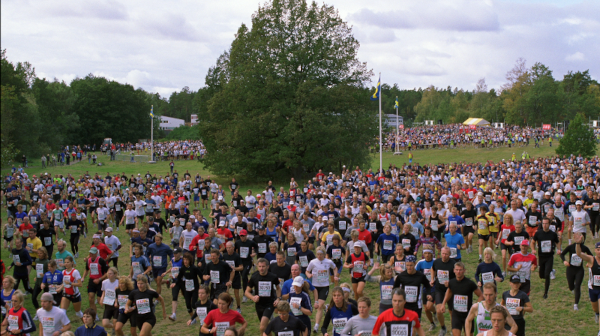
\includegraphics[height=0.4\textheight]{FIGURES/fig_36_1.png}
    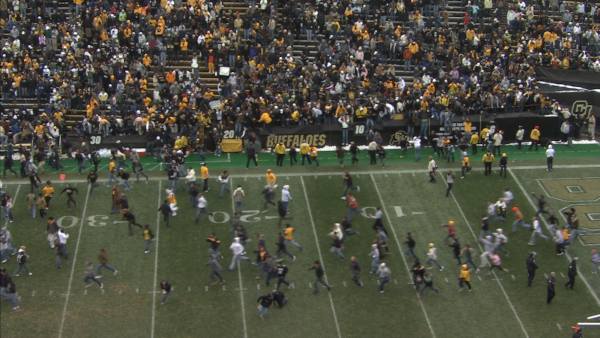
\includegraphics[height=0.4\textheight]{FIGURES/fig_36_2.png}
    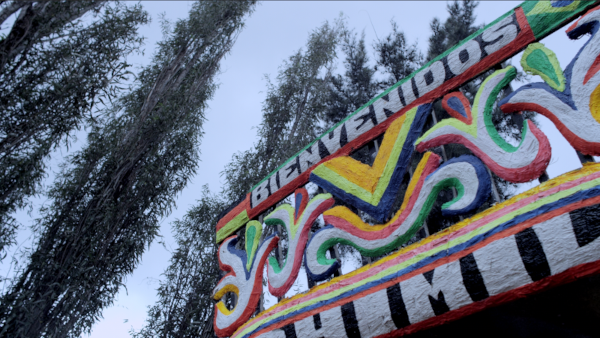
\includegraphics[height=0.4\textheight]{FIGURES/fig_36_3.png}
    \caption{Primeiro quadro das sequências HD1080 de maior destaque positivo em todos os experimentos, acima \textit{crowd\_run\_1080p50\_60f}, no meio \textit{rush\_field\_cuts\_1080p\_60f} e abaixo \textit{Netflix\_Boat\_1920x1080\_60fps\_8bit\_420\_60f}. Fonte: Elaborada pelo autor.}
    \label{fig:36}
\end{figure}
\end{landscape}
}

Desta forma, considerando tudo o que já foi abordado até o momento, é possível concluir que há sequências de vídeos em que as propostas de transcodificadores rápidos desenvolvidas apresentam resultados de redução de complexidade e impacto na eficiência de codificação dentro de valores desejáveis, como pode ser visto na Tabela \ref{tab:XXXVI}. Inclusive, as sequências com os resultados negativos nos mostram que há uma fragilidade na precisão do modelo implementado. Como apontado anteriormente, o uso da técnica de balanceamento de dados \textit{undersampling} aplica uma redução da capacidade de discernimento no limite entre decisões binárias. Desta forma, é preciso investigar e avaliar os melhores balanceamentos dos conjuntos de dados utilizados para treinamento e teste dos modelos, de forma a reduzir essa imprecisão entre particionar ou não particionar.

\afterpage{
\clearpage
\begin{landscape}
\begin{figure}
    \centering
    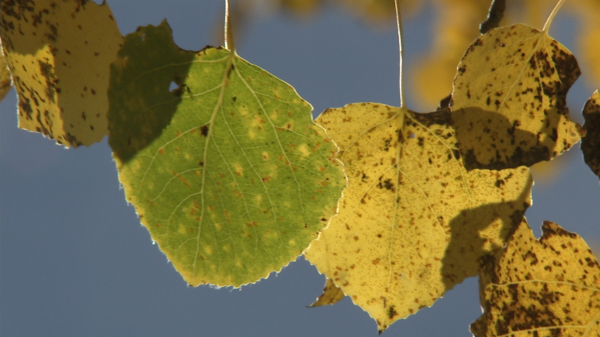
\includegraphics[height=0.4\textheight]{FIGURES/fig_37_1.png}
    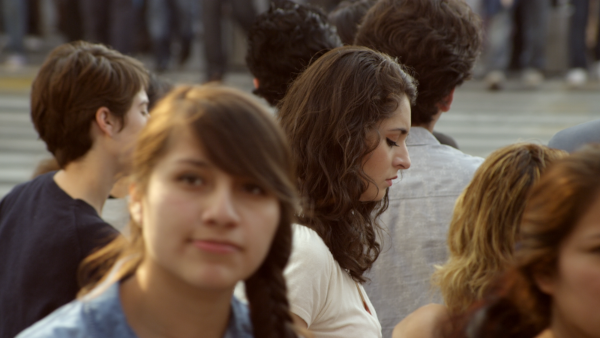
\includegraphics[height=0.4\textheight]{FIGURES/fig_37_2.png}
    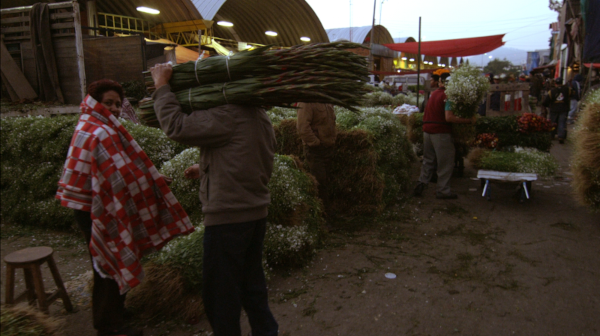
\includegraphics[height=0.4\textheight]{FIGURES/fig_37_3.png}
    \caption{Primeiro quadro das sequências HD1080 de maior destaque negativo em todos os experimentos, acima \textit{aspen\_1080p\_60f}, no meio \textit{Netflix\_Crosswalk\_1920x1080\_60fps\_8bit\_420\_60f} e abaixo \textit{Netflix\_FoodMarket\_1920x1080\_60fps\_8bit\_420\_60f}. Fonte: Elaborada pelo autor.}
    \label{fig:37}
\end{figure}
\end{landscape}
}

